\subsubsubsection{non-native-add}

\begin{enumerate}
    \item \verb|Target|: Check the additional relation among three non-native target objects.
    \item \verb|Constraints logic|:
    \begin{itemize}
        \item Check equation for gadget: \verb|a + b = c + modular * overflow|;
        \item Check that ``c < modular''.
    \end{itemize}
    \item \verb|Process layout|: See \ref{fig:non-native-add-layout}.
    \item \verb|Constraints info and costs|:
    \begin{itemize}
        \item gadget biguint-add num: 2
        \item gadget biguint-mul-by-bool num: 1
        \item gadget biguint-cmp num: 1
        \item gate type num: 3 (U32AddManyGate, ComparisonGate, ArithmeticGate)
        \item gate instance num: 23 = 3 (U32AddManyGate) + 16 (ComparisonGate) + 2 (ArithmeticGate (1,0)) + 1 (ArithmeticGate(1,-1)) + 1 (ArithmeticGate(1,1))
        \item copy-constraints: 186 = 32 * 2{biguint-add} + 9{biguint-mul-by-bool} + 9 + (4 + 9) * 8{biguint-cmp} = 186
    \end{itemize}
\end{enumerate}

\begin{figure}[!ht]
    \centering
    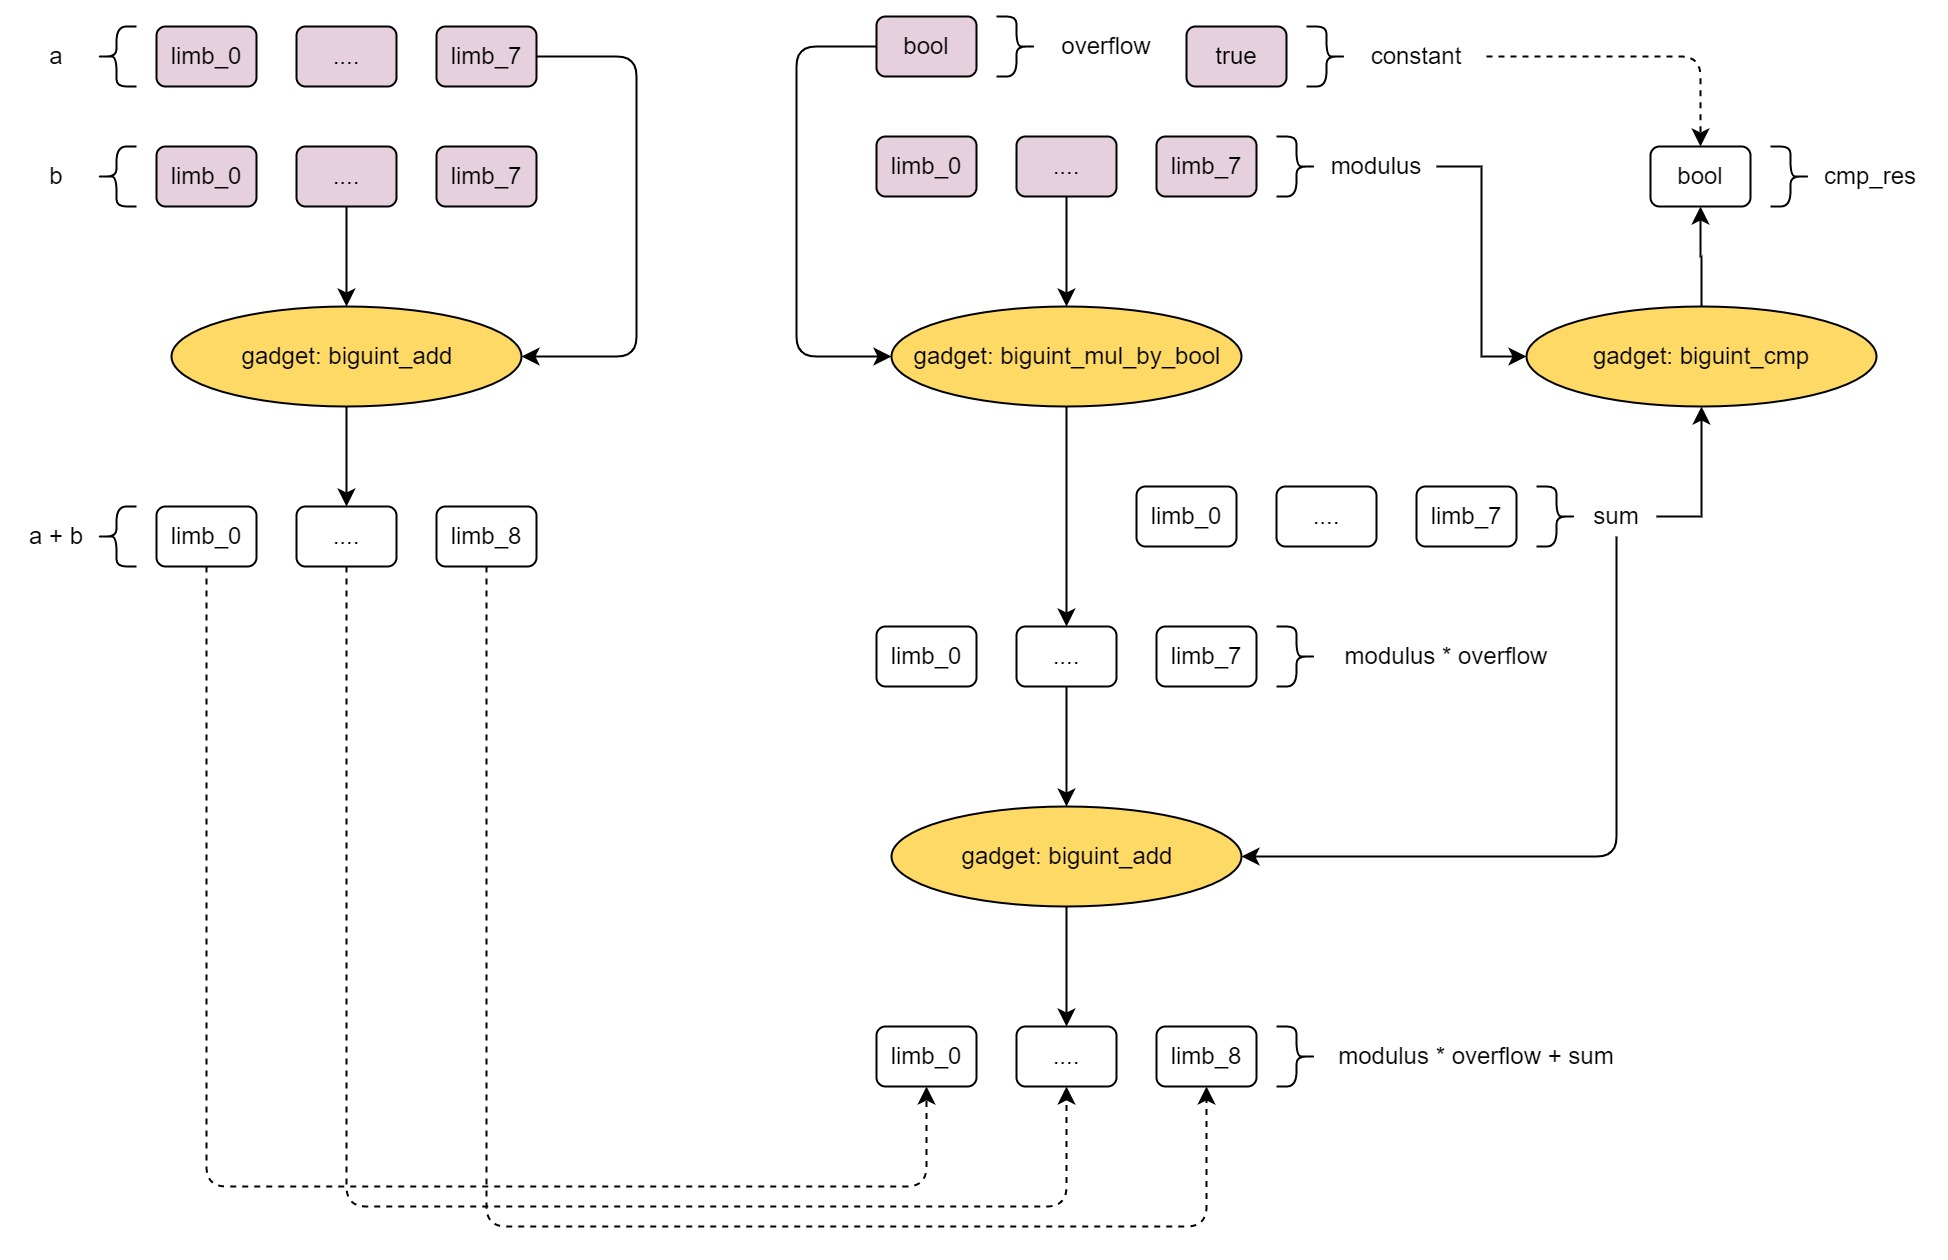
\includegraphics[width=0.6\textwidth]{nonnative-add-layout.jpg}
    \caption{non-native-add layout}
    \label{fig:non-native-add-layout}
\end{figure}
